\documentclass{standalone}

\usepackage{tikz}
\usetikzlibrary{arrows.meta}
\usetikzlibrary{positioning}

\begin{document}
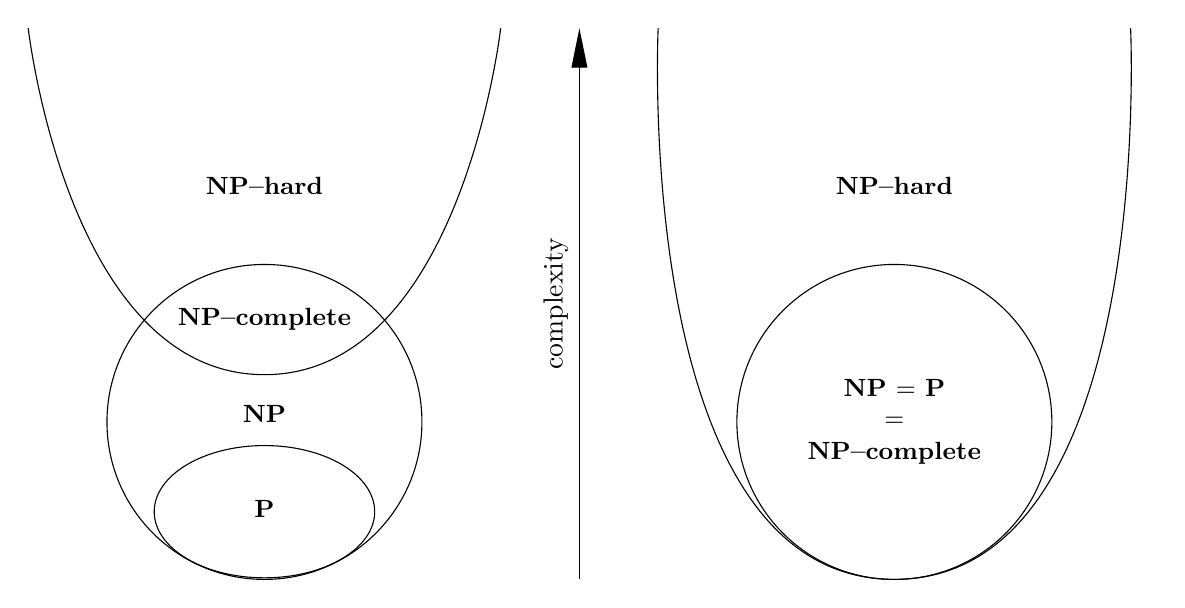
\begin{tikzpicture}

\draw (0, 0) circle [radius=2cm];
\draw (0,-1.14cm) ellipse (1.4cm and 0.84cm);
\draw plot [smooth, tension=1.5] coordinates { (-3,5) (0, 0.6) (3, 5)};
\node at (0, 0.1) (NP1) {\small\textbf{NP}};
\node at (0, -1.1) (P1) {\small\textbf{P}};
\node at (0, 1.3) (NPC1) {\small\textbf{NP--complete}};
\node at (0, 3) (NPH1) {\small\textbf{NP--hard}};

\draw (8, 0) circle [radius=2cm];
\draw plot [smooth, tension=2] coordinates { (5,5) (8, -2) (11, 5)};
\node at (8, 3) (NPH1) {\small\textbf{NP--hard}};
\node[text width=3cm, align=center] at (8, 0) (PNP) 
    {{\small\textbf{NP} = \textbf{P}\\=\\\textbf{NP--complete}}};

\draw[-{Triangle[length=5mm,width=2mm]}] 
    (4, -2) -- (4, 5) 
    node[midway, rotate=90, yshift=0.3cm] {complexity};
\end{tikzpicture}
\end{document}